\documentclass{article}
\usepackage[utf8]{inputenc}
\usepackage[a4paper, portrait, margin=1in]{geometry}
\usepackage{graphicx}
\usepackage{subcaption}
\usepackage{tabularx}
\usepackage{hyperref}
\hypersetup{
    colorlinks=true,
    linkcolor=blue,
    filecolor=magenta,      
    urlcolor=cyan,
}
\usepackage{amsmath}

\title{Cloud Computing (UE18CS352) \\Unit 4}
\author{Aronya Baksy}
\date{March 2021}

\begin{document}

\maketitle
\section{Master-Slave vs P2P Models}
\begin{itemize}
    \item Distributed System: A system that involves components on different physical machines that communicate, and coordinate actions in order to appear as a single system to the end user
    
    \item Two main types of distributed system architectures are \textbf{Master-Slave} and \textbf{Peer-to-Peer} (P2P)

\end{itemize}

\subsection{Master-Slave Architecture}
\subsubsection{Key Points}
\begin{itemize}
    \item Two types of nodes: master and worker
    
    \item Nodes are unequal, the master is above the worker nodes in the hierarchy. This makes the master a \textbf{single point of failure} (SPOF)
    
    \item The master is the \textit{central coordinator} of the system. All decisions regarding scheduling and resource allocation are made by master
    
    \item The master becomes a performance \textit{bottleneck} as the number of worker nodes increases. 
\end{itemize}
\begin{figure}[!ht]
    \begin{minipage}{0.45\textwidth}
        \centering
        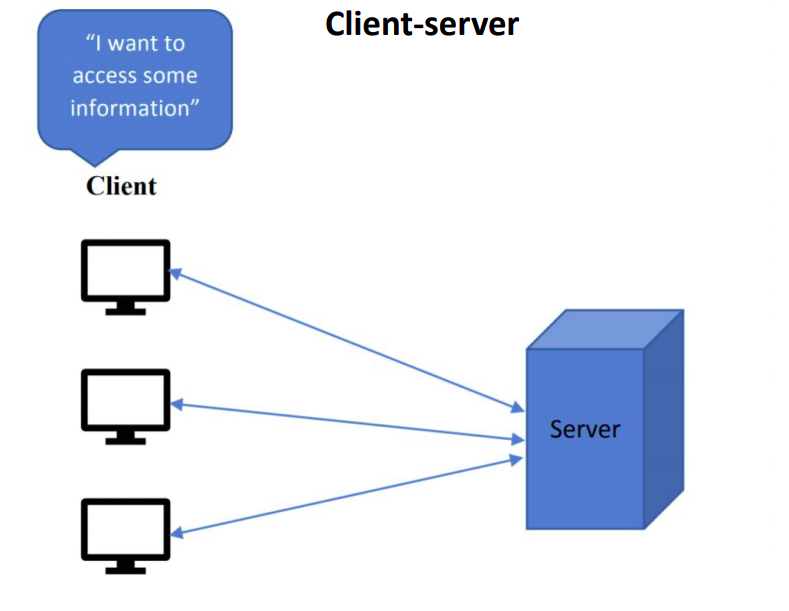
\includegraphics[width=0.9\textwidth]{cs.png} % first figure itself
        \caption{Client-Server Architecture}
    \end{minipage}\hfill
    \begin{minipage}{0.45\textwidth}
        \centering
        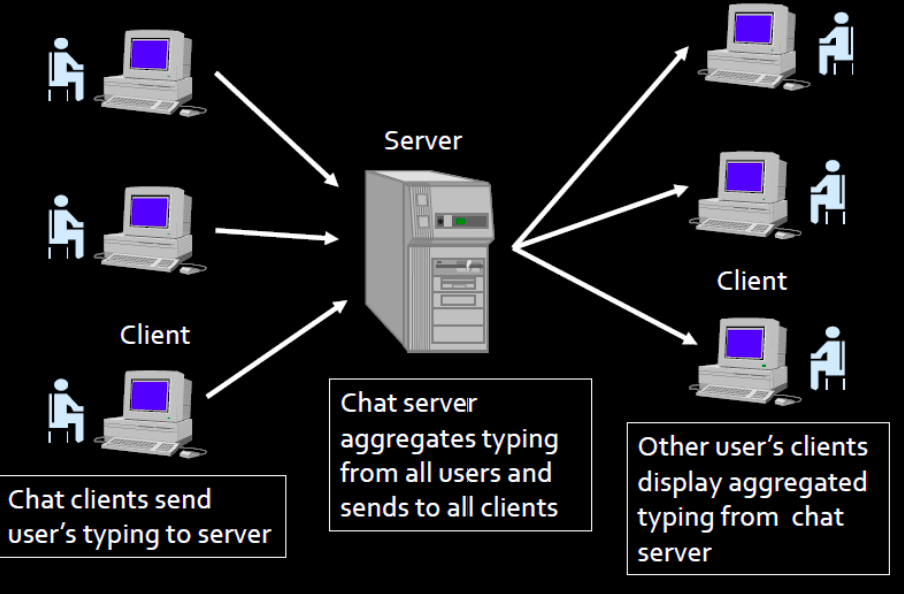
\includegraphics[width=0.9\textwidth]{chat.png} % second figure itself
        \caption{Client Server Model for Chat}
    \end{minipage}
\vfill 
    \begin{minipage}{0.45\textwidth}
        \centering
        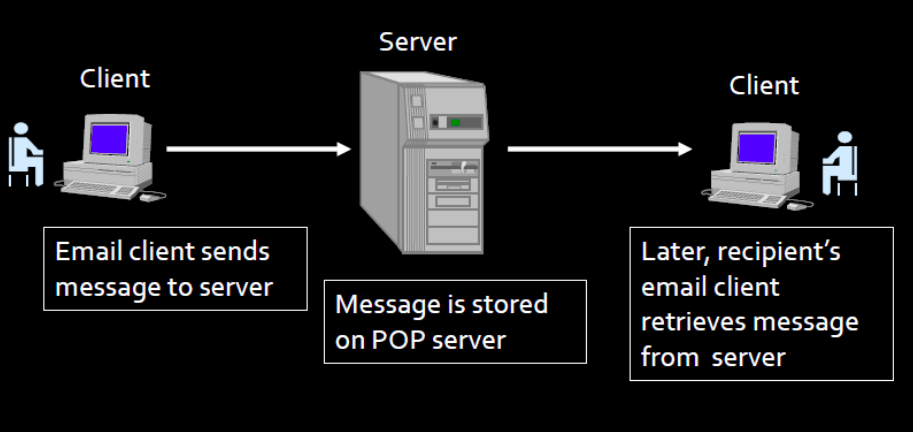
\includegraphics[width=0.9\textwidth]{email.png} % first figure itself
        \caption{Client-Server Architecture for e-mail applications}
    \end{minipage}\hfill
    \begin{minipage}{0.45\textwidth}
        \centering
        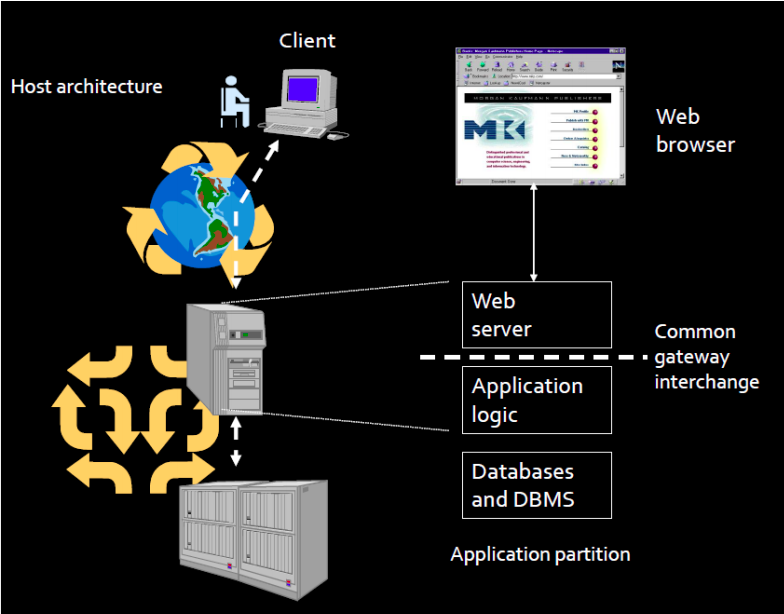
\includegraphics[width=0.9\textwidth]{webapp.png} % second figure itself
        \caption{3-tier Client Server Model}
    \end{minipage}
\end{figure}

\subsubsection{Advantages}
\begin{itemize}
    \item Easy maintenance and security
    
    \item Promotes sharing of resources and data between different h/w and s/w platforms
    
    \item Integration of services
\end{itemize}

\subsubsection{Disadvantages}
\begin{itemize}
    \item Not scalable as number of workers increase
    
    \item The master is a SPOF
\end{itemize}

\subsection{P2P Architecture}
\subsubsection{Key Points}
\begin{itemize}
    \item No hierarchical relationships between the nodes
    
    \item No central coordination, each node takes its own decisions on resource allocation. But synchronization of all the decisions is difficult.
    
    \item Theoretically $\infty$ scalability. No performance bottlenecks exist.
    
    \item Peers form groups and offer services/data within group members. Popular data is propagated within the group, unpopular data may die out. 
    
    \item Peers can form a Virtual Overlay Network on top of the physical topology. Each peer routes traffic through the overlay network.
\end{itemize}

\subsubsection{Advantages}
\begin{itemize}
    \item No centralized point of failure. 
    
    \item Highly scalable, addition of peers does not affect quality of service
\end{itemize}

\subsubsection{Disadvantages}
\begin{itemize}
    \item Maintaining decentralized coordination is tough (consistency of global state, needs distributed coherency protocols)
    
    \item Computing power and bandwidth of nodes impacts the performance (i.e. all nodes are not the same in a P2P network)
    
    \item Harder to program and build applications for P2P systems due to the decentralized nature.
\end{itemize}


\subsubsection{Applications}
\begin{itemize}
    \item \textbf{File Sharing} applications with replication for fault tolerance (e.g.: Napster, BitTorrent clients like $\mu$Torrent, Gnutella, KaZaa)
    
    \item Large-scale \textbf{scientific computing} for data analysis/mining (e.g.: SETI@Home, Folding@Home used for protein dynamics simulations)
    
    \item \textbf{Collaborative applications} like instant messaging, meetings/teleconferences (e.g.: IRC/ICQ, Google Meet, MS Teams etc.)
\end{itemize}

\subsection{P2P Topologies}
\subsubsection{Centralized Topology}
\begin{itemize}
    \item A centralized server must exist which is used to manage the files and user databases of multiple peers that log onto it
    
    \item The centralized server maintains a mapping between file names and IP addresses of a node. Each time a client joins the network, it publishes its IP address and list of files it shares to this database
    
    \item Any file lookup happens via the server. If the file is found then the centralized server establishes a direct connection with the requesting node and the node that contains the requested file.
\end{itemize}

\subsubsection{Ring Topology}
\begin{itemize}
    \item Consists of a cluster of machines that are arranged in the form of a ring to act as a distributed server. The ring provides better load balancing and high availability.
    
    \item Typically used when nodes are physically nearby, such as a single organization.
\end{itemize}

\subsubsection{Hierarchical Topology}
\begin{itemize}
    \item Suitable for systems that require a form of governance that involves delegation of rights or authority
    
    \item e.g.: DNS hierarchy, where authority flows from the root name servers to the servers of the registered name and so on
\end{itemize}

\subsubsection{Decentralized Topology}
\begin{itemize}
    \item All peers are equal, hence creating a flat, unstructured network topology 
    
    \item In order to join the network, a peer must first, contact a bootstrapping node (node that is always online), which gives the joining peer the IP address of one or more existing peers.
    
    \item Each peer, however, will only have information about its direct neighbours. 
    
    \item Any file queries have to be flooded to all the nodes in the network. 
    
    \item e.g.: GNutella, for file sharing especially music
\end{itemize}

\begin{figure}[!ht]
    \begin{minipage}{0.45\textwidth}
        \centering
        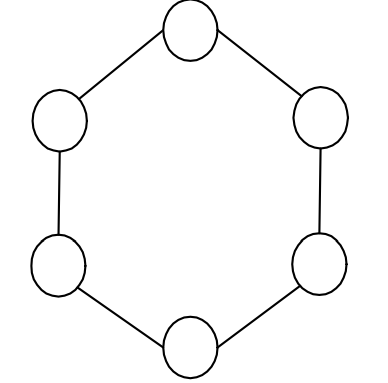
\includegraphics[scale=0.3]{ring.png} % first figure itself
        \caption{Ring Topology}
    \end{minipage}\hfill
    \begin{minipage}{0.45\textwidth}
        \centering
        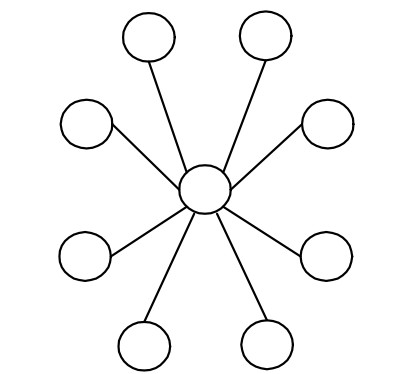
\includegraphics[scale=0.3]{central.png} % second figure itself
        \caption{Centralized Topology}
    \end{minipage}
\vfill 
    \begin{minipage}{0.45\textwidth}
        \centering
        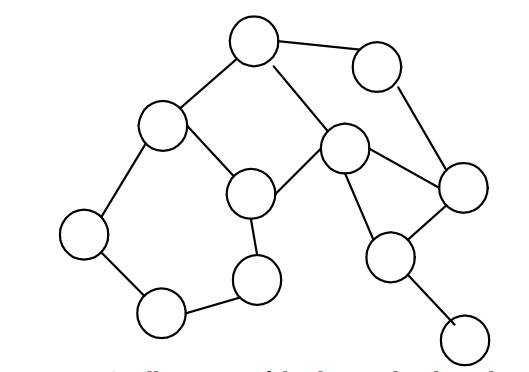
\includegraphics[scale=0.3]{decentralized.png} % first figure itself
        \caption{Decentralized Topology}
    \end{minipage}\hfill
    \begin{minipage}{0.45\textwidth}
        \centering
        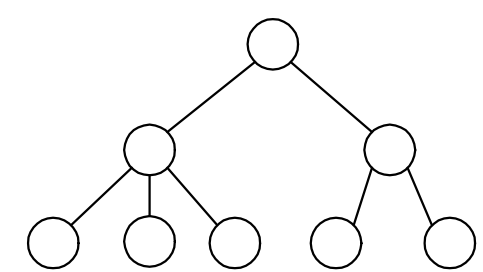
\includegraphics[scale=0.3]{hierarchical.png} % second figure itself
        \caption{Hierarchical Topology}
    \end{minipage}
\end{figure}

\section{Unreliable Communication}
\begin{itemize}

    \item Issues with communication in distributed systems:
    \begin{itemize}
        \item Request or response is lost due to issues in the interconnect network 
        \item Delay in sending request or response (due to queuing delays and network congestion)
    
        \item Remote node failure (permanent or temporary)
    \end{itemize}
    
    \item \textit{Partial Failure} in a distributed system occurs when some components (not all) start to function \textit{unpredictably}. Partial failures are \textit{non-deterministic}.
    
    \item Distributed systems involve accepting partial failure, building fault-tolerant mechanisms into the system.
    
    \item \textbf{Reliability} is the ability of a system to continue normal functioning even when components fail or other issues occur. 
    
    \item Formally, reliability is defined as the probability that a system meets certain performance standards and yields correct outputs over a desired period of time
    
    \item Reliability includes:
    \begin{itemize}
        \item Tolerant to unexpected behaviour and inputs in the software
        
        \item Prevention of unauthorized access and abuse
        
        \item Adequate performance for the given use case under expected load and input size
    \end{itemize}
    
    \item Metric for reliability: \textbf{mean time between failures}, defined as
    \begin{equation*}
        MTBF = \frac{\text{total uptime}}{\text{\# of failures}}
    \end{equation*}
    
    \item A fault is usually defined as one component of the system deviating from its spec
    
    \item A failure is when the system as a whole stops providing the required service to the user
    
    \item Fault-tolerant mechanisms prevent faults from causing system-wide failures. 
    
    \item Classification of faults:
    \begin{itemize}
        \item \textbf{Transient}: appear once, then vanish entirely (e.g. first request from node A to node B fails to reach, but the next one reaches on time)
        
        \item \textbf{Intermittent}: Occurs once, vanishes, but reappears after a random interval of time. (e.g. loose hardware connections)
        
        \item \textbf{Permanent}: Occurs once, interrupts the functioning of the system until it is fixed. (e.g. infinite loops or OOM errors in software)
    \end{itemize}
    
    \item Classification of failures:
    \begin{itemize}
        \item \textbf{Crash failure}: A server halts, but functions correctly till that point
        
        \item \textbf{Omission Failure}: Could be send omission (server fails to send messages) or receive omission (server fails to respond to incoming messages)
        
        \item \textbf{Timing Failure}: server response is delayed beyond the acceptable threshold
        
        \item \textbf{Response Failure}: Could be a value failure (response value is wrong for a request) or a state transition failure (deviation from correct control flow)
        
        \item \textbf{Arbitrary or Byzantine Failure}: Arbitrary response produced at arbitrary times
    \end{itemize}
\end{itemize}

\subsection{Failure Detection}
\begin{itemize}
    \item Using \textbf{timeout}: Let $d$ be the longest possible delivery time (all messages will reach within time $d$ after being sent or they will not reach at all), and $r$ be the time needed by the server to process the message. 
    
    \item Then the round trip time $2d+r$ is a reasonable estimate for a timeout value beyond which it can be assumed that a node has failed. 
    
    \item Unfortunately, there are no such time guarantees in asynchronous communications that are used in distributed systems. 
    
    \item Network congestion causes queuing delays. If queues fill up at routers, then the packets can be dropped, causing retransmission and further congestion
    
    \item Even VMs that give up control of the CPU core to another VM can face network delays as they stop listening to the network for that short duration when they are not in control of the CPU. This leads to packets dropping. 
    
    \item Timeout values are measured \textit{experimentally}. 
    \begin{itemize}
        \item Data is collected on round-trip times across multiple machines in the network and over an extended time period. Measure the variability in the delays (aka \textbf{jitter})
        
        \item Taking into account this data, as well as the application characteristics, a timeout is chosen that is a fair compromise between delay in failure detection and premature timeout.
        
        \item Instead of constant timeouts, the system constantly measures response time and jitter, and dynamically adjusts the timeout value.
        
        \item This is used in Phi Accrual Failure Detector in systems like Cassandra and Akka (toolkit for distributed applications in Java/Scala)
    \end{itemize}
    
    \item In circuit switched networks, there is no queuing delay as the connection is already set up end-to-end before message exchange, and the maximum end-to-end latency of the network is fixed (bounded delay)
    
    \item The disadvantage of circuit switched network is that it supports far less number of concurrent network users, and it leads to low bandwidth utilization. 
\end{itemize}

\subsection{Failure Models}
\begin{itemize}
    \item \textbf{Fail-Stop}: Assumes that nodes can fail only by crashing. Once a node stops responding it never responds until it is brought back online
    
    \item \textbf{Fail-Recovery}: Once a node stops responding it may start responding again after a random time interval. Nodes are assumed to have stable disk storage that persists across failures, but in-memory state is assumed to be lost
    
    \item \textbf{Byzantine}: A component such as a server can inconsistently appear both failed and functioning to failure-detection systems, showing different symptoms to different observers.
\end{itemize}

\subsection{Byzantine Faults}
\begin{itemize}
    \item A Byzantine fault is a condition of a distributed system where components may fail and there is imperfect information on whether a component has failed. 
    
    \item A system is said to be Byzantine fault-tolerant if it continues to work properly despite nodes not obeying correct protocol, or if malicious actors are interfering with the working of the system
    
    \item The Byzantine agreement:
    \begin{itemize}
        \item Used to build consensus that nodes have failed or messages are being corrupted
        
        \item General strategy is to have each node communicate not only its own status but any information they have on any other nodes. 
        
        \item Using this information, a majority consensus is built and the nodes that don't agree with this consensus are considered to be in failure state.
    \end{itemize}
\end{itemize}

\subsection{Failure Detection using Heartbeats}
\begin{itemize}
    \item A heartbeat is a signal sent from a node to another at a fixed time interval that indicates that the node is alive. 
    
    \item Absence of a fixed number of consecutive heartbeats from a node is assumed to be evidence that that node is dead
    
    \item Heartbeat signals are organized in the following ways:
    \begin{itemize}
        \item \textbf{Centralized}: All nodes send heartbeats to a central monitoring service. Simplest organization but the central service is now a SPOF
        
        \item \textbf{Ring}: Each node sends heartbeat only to one neighbour, forming a ring structure. If one of the nodes fails, then the ring breaks and heartbeats cannot be sent properly
        
        \item \textbf{All-to-All}: Each node sends heartbeats to every other node in the system. High communication cost but every node keeps track of all other nodes hence high fault tolerance.  
    \end{itemize}
\end{itemize}

\subsection{Failover}
\begin{itemize}
    \item The act of switching over from one service/node/application to a new instance of the same, upon the failure or abnormal termination of the first one. 
    
    \item Failover can be implemented in two ways:
\end{itemize}
\subsubsection{Active-Active Failover Architecture}
\begin{itemize}
    \item Also called symmetric failover. 
    
    \item Let there be 2 servers. Server 1 runs application A and server 2 runs application B. If server 1 fails for some reason, then server 2 will now be tasked with running both applications A and B. 
    
    \item Since the databases are replicated, it mimics having only one instance of the application, allowing data to stay in sync.
    
    \item This scheme is called Continuous Availability because more servers are waiting to receive client connections to replicate the primary environment if a failover occurs.
\end{itemize}
\begin{figure}[!h]
    \centering
    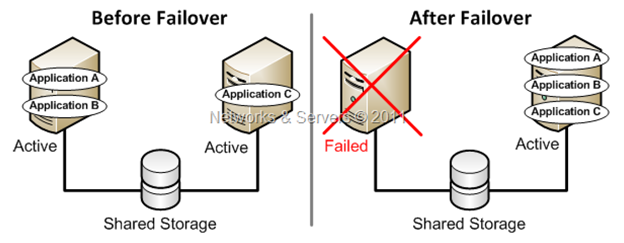
\includegraphics[scale=0.6]{active-active.png}
    \caption{Active-Active Failover Architecture}
    \label{fig:my_label_69}
\end{figure}

\subsubsection{Active-Passive Failover Architecture}
\begin{itemize}
    \item Also called asymmetric failover.
    
    \item A standby server is configured to take over the tasks run by the active primary server, but otherwise the standby does not perform any functions. 
    
    \item The server runs on the primary node until a failover occurs, then the single primary server is restarted and relocated to the secondary node.
    
    \item Not necessary to shift functions back to the primary server once it comes back online (called failback). In this situation the primary is the new standby, and the previous standby is currently the primary. 
\end{itemize}

\begin{figure}[!ht]
    \centering
    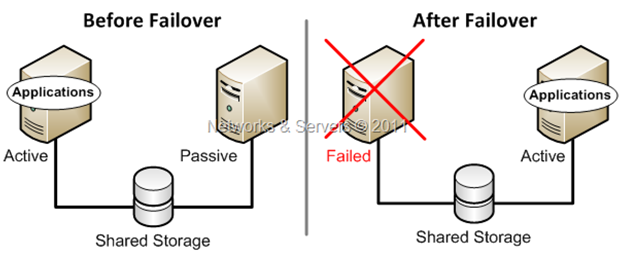
\includegraphics[scale=0.6]{active-passive.png}
    \caption{Active-Passive Failover Architecture}
    \label{fig:my_label_6969}
\end{figure}

\section{Availability and Fault Tolerance}
\subsection{Availability}
\begin{itemize}
    \item Availability is used to describe the situation where a service is ready to respond to user requests, as well as the time spent in actually servicing those requests.
    
    \item Uptime refers to the period during which a service is operational. Downtime refers to the period during which a service in unavailable and non-operational. 
    
    \item Most modern distributed systems give an uptime guarantee of 99.999\% (5 nines).
    
    \item Downtime may be planned (maintenance is generally planned beforehand at regular intervals) or unplanned (due to network outages, node failures, software crashes)
    
    \item The \textbf{Service Level Agreement} (SLA) between the cloud provider and end user includes an uptime-downtime ratio. 
    
    \item Available systems are generally designed by eliminating as many SPOF as possible. As size of system increases, isolation of faults becomes harder hence availability reduces. 
    
    \item Most distributed systems have \textbf{high availability with failover}. 
\end{itemize}

\begin{figure}[!h]
    \centering
    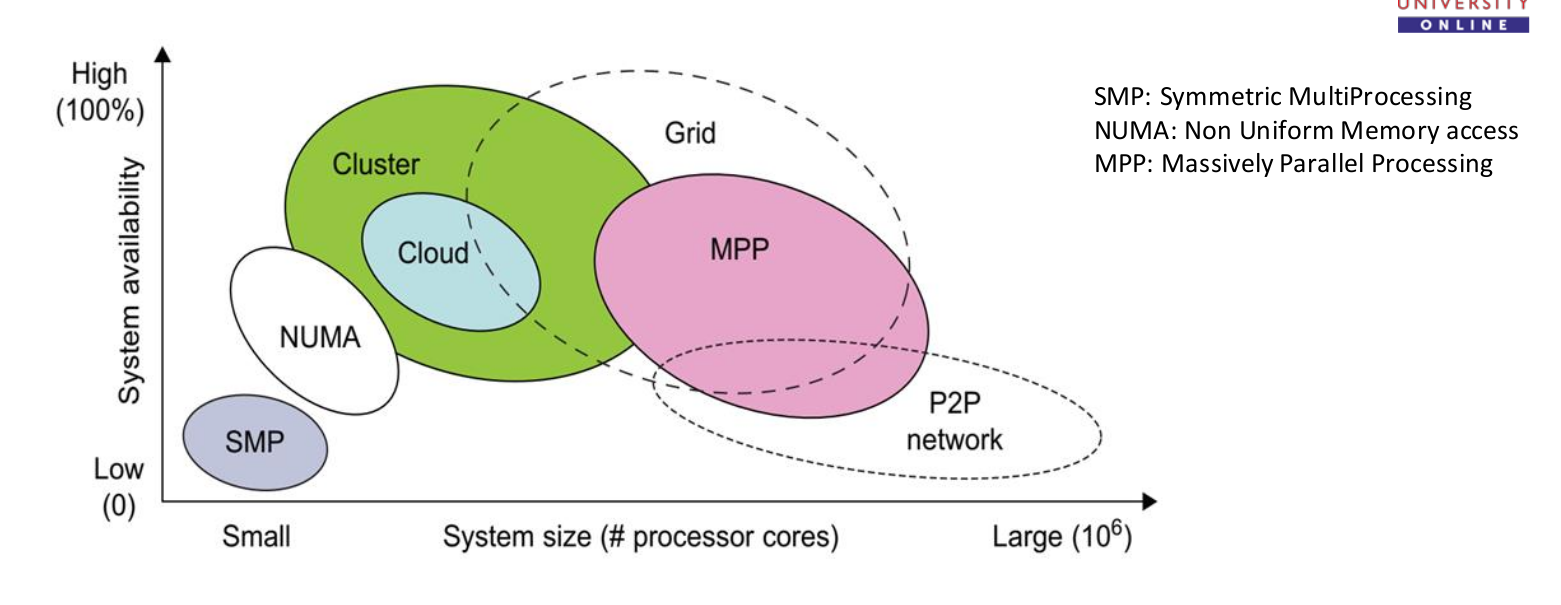
\includegraphics[scale=0.3]{pic1.png}
    \caption{Availability for different types of distributed systems}
    \label{fig:my_label_69696969}
\end{figure}
\begin{itemize}
    \item Availability is measured in terms of the following metrics:
\end{itemize}

\subsubsection{Mean Time to Failure (MTTF)}
\begin{itemize}
    \item Measured as
    \begin{equation}
        MTTF = \frac{\text{Total uptime}}{\text{Number of tracked operations/components}}
    \end{equation}
    
    \item It is a measure of failure rate of a product
    
    \item MTTF is only used for \textbf{non repairable, only replacable} components (such as motherboards, memory, disk drives, batteries etc.)
\end{itemize}

\subsubsection{Mean Time to Repair (MTTR)}
\begin{itemize}
    \item Measured as
    \begin{equation}
        MTTR = \frac{\text{Total downtime caused by failures}}{\text{Number of failures}}
    \end{equation}
    
    \item It measures the average time to repair and restore a failed system
\end{itemize}

In terms of the above metrics, the system availability is defined as:
\begin{equation}
    Availability = \frac{MTTF}{MTTF + MTTR}
\end{equation}

\subsection{Fault Tolerance}
\begin{itemize}
    \item Ability of system to continue operation without interruption, despite failure of one or more components. 
    
    \item Fault tolerance can be implemented either in hardware (duplicate hardware), or in software (duplicate instances running the same software) or using load balancers (redirect traffic away from failed instances). 
    
    \item Fault tolerant architectures, however, do not address software failures which are the most common cause of downtime in real-life distributed systems. 
\end{itemize}

\begin{tabular}{|p{0.2\textwidth}|p{0.35\textwidth}|p{0.35\textwidth}|}
    \hline 
    \textbf{Consideration} & \textbf{Highly Available} & \textbf{Fault Tolerant} \\
    \hline
    \textbf{Downtime} & Minimal allowed downtime for service interruption (e.g. 99.999\% uptime means 5 mins downtime per year) & Zero downtime, continuous service expected \\
    \hline
    \textbf{Cost} & Less expensive to implement as no redundant hardware is needed & More expensive to implement as it requires redundant components \\
    \hline
    \textbf{Scope} & Use shared resources to manage failures and minimize downtime & Use power supply backup, components that can detect failure and automatically switch over to redundant components \\
    \hline
    \textbf{Example} & e.g.: Non-critical software and IT services (Amazon etc.) & e.g.: Critical applications (related to healthcare, defense etc.) \\
    \hline
\end{tabular}

\subsection{Implementation of Fault Tolerance}
\begin{itemize}
    \item Hardware systems backed by equivalent components. Replicate data and compute functions between redundant servers
    
    \item Build fault-tolerance into network architecture. Multiple paths between nodes in a data-center, or mechanisms to handle link failure and switch failure
    
    \item Handle link failures transparently without affecting cloud functionality. Avoid forwarding packets on broken links. 
    
    \item Redundant power supply using generators. 
    
    \item Software instances are made fault tolerant by setting up duplicate instances. (e.g. if DB is running and it fails, switch to another instance of the same DB running on another machine)

\end{itemize}

\subsubsection{Chaos Monkey}
\begin{itemize}
    \item Chaos Monkey is a suite of tools designed by engineers at Netflix designed to randomly introduce failures in a production environment.  
    
    \item Chaos Monkey is used to purposefully introduce faults into systems that are under development so that fault tolerance can be integrated as early as possible and tested at any time. 
    
    \item By regularly "killing" random instances of a software service, it is possible to test a redundant architecture to verify that a server failure does not noticeably impact customers.
    
    \item Chaos Monkey relies on Spinnaker (an open source CI/CD tool similar to Jenkins) that can be deployed on all major cloud providers (AWS, Google App Engine, Azure)
    
    \item The suite of tools developed by Netflix under this includes:
    \begin{itemize}
        \item \textbf{Chaos Kong}: Drop an entire AWS Region
        
        \item \textbf{Chaos Gorilla}: Drop an entire AWS Availability Zone
        
        \item \textbf{Latency Monkey}: Introduces delays to simulate network outages or congestion
        
        \item \textbf{Doctor Monkey}: Monitor performance metrics, detect unhealthy instances, for analysis of root causes and eventual fixing/retirement of the instance.
        
        \item \textbf{Janitor Monkey}: Identify and clean unused instances 
        
        \item \textbf{Conformity Monkey}: Identifies non-conforming instances according to a set of rules (age of instances, security groups of clustered instances etc.)
        
        \item \textbf{Security Monkey}: Search for and delete instances with known security vulnerabilities and invalid config
        
        \item \textbf{10-18 Monkey} Detects problems with localization and internationalization for software serving customers across different geographic regions.
    \end{itemize}
\end{itemize}


\subsection{Fault Tolerant Design Patterns for Microservice Architectures}
\subsubsection{Use Asynchronous Communication}
\begin{itemize}
    \item Avoid long chains of synchronous HTTP calls when communicating between services as the incorrect design leads to major outages. 
    
    \item This helps minimize ripple effects caused by network outages.
\end{itemize}

\subsubsection{Work around Network Timeouts}
\begin{itemize}
    \item To ensure that reosurces are not indefinitely occupied, use network timeouts.
    
    \item Clients should be designed not to block indefinitely and to always use timeouts when waiting for a response
\end{itemize}

\subsubsection{Retry with Exponential Backoff}
\begin{itemize}
    \item Perform retries to service calls at exponentially increasing intervals. 
    
    
    \item This is done to counter intermittent failures when the service is only unavailable for short time. 
    
    \item Microservices should be designed with circuit breakers so that the increased network load due to the successive retries does not cause Denial of Service (DoS)
\end{itemize}

\subsubsection{Circuit Breaker Pattern}
\begin{itemize}
    \item In this approach, the client process tracks the number of failed requests. 
    
    \item If the error rate exceeds a configured limit, a "circuit breaker" trips so that further attempts fail immediately. (large number of failed requests implies that the service is unavailable, hence don't contact now)
    
    \item After a timeout period, the client should try again and, if the new requests are successful, close the circuit breaker.
\end{itemize}

\begin{figure}[!ht]
    \centering
    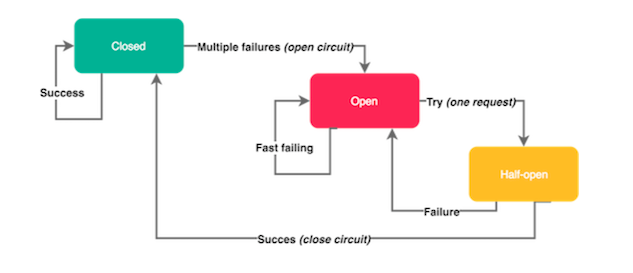
\includegraphics[scale=0.5]{ckt_break.png}
    \caption{Circuit Breaker Design Pattern}
    \label{fig:my_label_4761}
\end{figure}

\subsubsection{Fallback Mechanisms}
\begin{itemize}
    \item Fallback provides an alternative solution during a service request failure. 
    
    \item Fallback logic is implemented that runs when a request fails. The logic may involve returning a default value, or returning some cached value.
    
    \item Fallback logic must be simple and failure-proof as it is itself running due to a failure. 
\end{itemize}

\begin{figure}[!h]
    \centering
    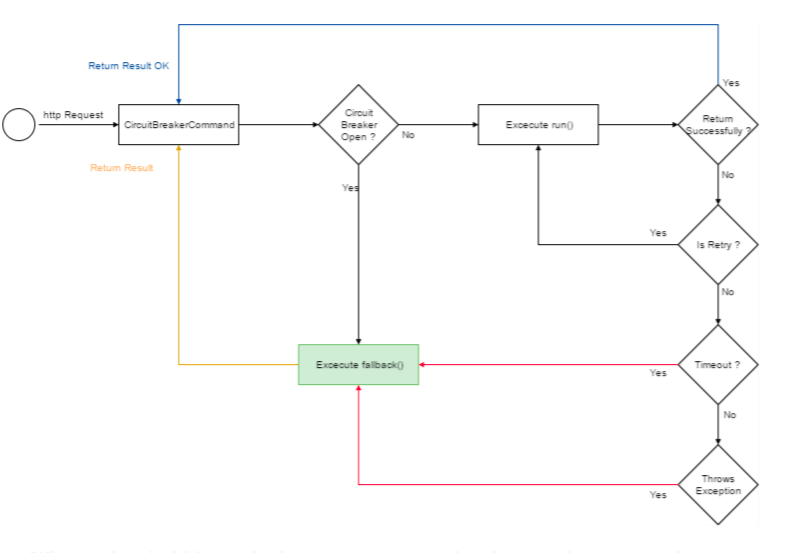
\includegraphics[scale=0.4]{fallback.png}
    \caption{Circuit Breaker Pattern with fallback logic}
    \label{fig:my_label}
\end{figure}

\subsubsection{Limit number of queued requests}
\begin{itemize}
    \item Clients impose an upper bound on number of outstanding requests that can be sent to a service. 
    
    \item In case this upper bound is crossed, the remaining requests should automatically fail. 
    
    \item This is a form of rate limiting or throttling, controlling the rate of requests sent in a time period
    
    \item If request arrival rate exceeds the processing rate, the incoming requests can either be queued in a FIFO queue, or discarded when the queue fills up. 
    
    \item When the service has capacity, it retrieves messages from this queue and processes them. When the request rate is greater, the available capacity messages are processed in order and are not lost. 

\end{itemize}

\section{Task Scheduling Algorithms}
\begin{itemize}
    \item Policies that assign tasks to the appropriate available resources (CPU, Memory, bandwidth) in a manner that ensures maximum possible utilization of those resources
    
    \item Categorized into:
    \begin{itemize}
        \item \textbf{Immediate} scheduling algorithms assign tasks to VMs as soon as they arrive
        
        \item \textbf{Batch} schedulers group tasks into batches and schedule individual batches onto VMs
        
        \item \textbf{Static} schedulers do not take into account the current state of the system, but rather use only prior available information on the state. Divides all traffic equally among all VMs, e.g. round robin or random scheduling.
        
        \item\textbf{Dynamic} schedulers take into account the current system, do not need any prior information on the system, and distribute tasks as per the relative capacities of the VMs
        
        \item \textbf{Preemptive} scheduling means that tasks can be interrupted and moved to other resources where they can continue execution
        
        \item \textbf{Non-preemptive} scheduling means that a task cannot be reallocated to a new VM until its execution is complete
    \end{itemize}
    
    \item Levels of task scheduling:
    \begin{itemize}
        \item The \textbf{Task level}. Consists of tasks or cloudlets sent to the system by the users
        
        \item The \textbf{scheduling level}. It is responsible for mapping tasks to resources to get highest resource utilization with minimum completion time for all tasks (aka minimum makespan)
        
        \item The \textbf{VM level}. Consists of VMs that execute the scheduled tasks
    \end{itemize}
\end{itemize} 


\subsection{FCFS Scheduling}
\begin{itemize}
    \item Advantage: Simplest to implement and understand. 
    
    \item Drawback: Leads to longer wait times and lower resource utilization
    
    \item Algorithm: Assign tasks to VMs in the order of their arrival time. If more tasks than VMs then assign tasks in a round-robin manner.
\end{itemize}

\subsection{SJF Scheduling}
\begin{itemize}
    \item Advantage: Lowest average wait time among all algorithms (provably optimal). 
    
    \item Drawback: Long tasks are forced to wait for long times (starvation), and cannot be implemented at the short-term level. 
    
    \item Algorithm: Sort all available tasks in increasing order of their execution time. Then assign the tasks to VMs in sequential order of the VMs.
\end{itemize}

\subsection{Min-Max Scheduling}
\begin{itemize}
    \item Advantage: Efficient resource utilization
    
    \item Drawback: Leads to increased waiting time for small and medium tasks
    
    \item Algorithm: Sort tasks in decreasing order of execution time (longest task first). Sort VMs in decreasing order of performance (most powerful VM first, i.e. VM with minimum latency first). Now assign tasks to VM in order. 
\end{itemize}

\section{Cluster Coordination}
\begin{itemize}
    \item Consensus is the task of getting all processes in a group to agree on a single value based on votes gathered from all processes. The value agreed upon has to be submitted by one of the processes, i.e. this value cannot be invented by the consensus algorithm
    
    \item Synchronous processes are those that follow a common clock, while asynchronous processes are those where each process has an individual clock. 
    
    \item In asynchronous systems, it is not possible to build a consensus algorithm as it is impossible to distinguish between processes that are dead, and those are just slow in responding.
    
    \item If even one process crashes in an asynchronous system, then the consensus problem is \textbf{proved} to be unsolvable in \href{http://groups.csail.mit.edu/tds/papers/Lynch/jacm85.pdf}{this paper} by Fischer, Lynch and Patterson from 1985.
    
    \item Why solve consensus? It is important because many problems in distributed computing take a similar form to the consensus problem such as:
    \begin{itemize}
        \item Leader election
        
        \item Perfect failure detection
        
        \item Mutual exclusion (agreement on which node gets access to a particular shared resource)
    \end{itemize}
    
    \item The \textbf{properties} to be satisfied by asynchronous consensus are:
    \begin{itemize}
        \item \textbf{Validity}: The system cannot accept any value that was not proposed by atleast one node. If every node proposes the same value then that value is accepted
        
        \item \textbf{Uniform Agreement}: No two correct processes can agree on different values after a single complete run of the algorithm
        
        \item \textbf{Non-Triviality/Termination}: All the processes must eventually agree on a single value 
    \end{itemize}
\end{itemize}

\subsection{Consensus Algorithm: Paxos}
\subsubsection{Roles in Paxos}
\begin{itemize}
    \item Every node in a Paxos system is either a \textbf{proposer}, a \textbf{acceptor} or a \textbf{learner}.
    
    \item \textbf{Proposers} try to convince the acceptors that the value proposed by them is correct
    
    \item \textbf{Acceptors} receive proposals from proposers. They also inform the proposer in the event that a value other than the one proposed by them was accepted
    
    \item \textbf{Learners} announce the outcome of the voting process to all the nodes in the distributed system. 
\end{itemize}

\subsubsection{Paxos Phase 1 (Prepare - Promise)}
\begin{itemize}
    \item Every proposer creates a \textbf{prepare message} containing the node ID of the proposer (node ID is a single positive integer, monotonically increasing and unique to a single node), as well as the value proposed. 
    
    \item This message is sent to a majority of the acceptors. 
    
    \item If the acceptor has never seen any prepare message before, it sends back a \textbf{prepare response} message which indicates that the acceptor promises not to accept any prepare with an ID less than the current one. 
    
    \item In case the acceptor has seen a message before, it compares the ID in the incoming prepare message with the max ID it has seen. 
    \begin{itemize}
        \item If current ID is greater than max ID, then it sends back a \textbf{prepare response}. This promise message contains the Id and value of the highest previously accepted message. The promise is made not to accept any prepare message with ID less than current ID. 
        
        \item If current ID is smaller than max ID then simply ignore the current prepare message
    \end{itemize}
\end{itemize}

\subsubsection{Paxos Phase 2 (Propose - Accept)}
\begin{itemize}
    \item Once a proposer receives a prepare response from a majority of the acceptors, it can start sending out accept requests. 
    
    \item A proposer sends out an accept request containing its node ID, and the highest value it recevied from all the prepare responses. 
    
    \item If an acceptor receives an accept request for a higher or equal ID than it has already seen, it accepts and sends a notification to every learner
    
    \item A value is chosen by the Paxos algorithm when a learner discovers that a majority of acceptors have accepted a value.
\end{itemize}


\subsection{Leader Election Algorithms}
\begin{itemize}
    \item Elect a single leader from a group of non-faulty processes such that all processes agree on who the leader is
    
    \item Leader election criteria:
    \begin{itemize}
        \item Any process can call for an election, but a process can call for only one election at a time
        
        \item Multiple processes can call an election simultaneously. The result of all these elections is the same
        
        \item Result of an election does not depend on which process called the election
    \end{itemize}
    
    \item Conditions for successful leader election run:
    \begin{itemize}
        \item \textbf{Safety}: Every non faulty process $p$ must either elect a process $q$ with the best attribute value, or NULL
        
        \item \textbf{Liveness}: An election, once started, must terminate, and the result of a terminated election cannot be NULL. 
    \end{itemize}
    
    \item Each node has an attribute value which is its identifier. The value determines that node's fitness for leadership. (e.g.: CPU power, disk space, etc.)
\end{itemize}

\subsubsection{Ring Election}
\begin{itemize}
    \item All $N$ nodes are arranged in a logical ring. The node $p[i]$ has a direct link to the next node $p[(i+1) mod N]$
    
    \item Messages are only sent in clockwise order around the ring. The node that discovers the failure of the existing coordinator starts the process of election by sending its attribute value in an \textbf{election} message to the next node.
    
    \item Algorithm: 
    \begin{itemize}
        \item When a node receives an election message, it checks the attr value in that message. 
        
        \item If the incoming attribute value is less than the node's attribute value, the node overwrites the message with its own attribute value and sends it to the next node in the ring.
        
        \item If the incoming attribute value is greater than the node's attribute value, the node simply forwards the message to the next node in the ring. 
        
        \item If the incoming attribute value happens to the same as the node's attribute value, the election stops. The newly elected leader sends out \textbf{elected messages} to the next node, which forwards them to the next node and so on until all nodes in the ring have received an elected message containing the leader's ID. 
    \end{itemize}
    
    \item Worst case occurs when the leader is the anti-clockwise neighbour of the initiator. In this case the \textit{number of messages exchanged} is $3N - 1$ ($N-1$ election messages to reach the leader, $N$ election messages to confirm that no higher node exists and finally $N$ elected messages) 
    
    \item The simple ring election algorithm offers safety and liveness as long as nodes don't crash during election. 
    
    \item If the nodes crash during election, then it could lead to an election message going around the ring infinitely, thus the election goes on forever and liveness is not followed.
\end{itemize}

\subsubsection{Modified Ring Election}
\begin{itemize}
    \item Similar set up to the simple ring election case. 
    
    \item Algorithm:
    \begin{itemize}
        \item The initiator sends out an \textbf{election message} to the next running node in the ring. The first message contains the attr value of the initiator. 
        
        \item If a node receives an election message, it simply appends its own attribute value to the message and forwards it back. 
        
        \item When the election message completes one round and reaches the initiator again, the initiator selects the process with the best attribute value and crafts a \textbf{coordinator message}. 
        
        \item The \textbf{coordinator message} is of the form $coord(n_i)$ where $n_i$ is the elected node value. The coordinator message is sent around the ring, each node appends its own attribute value to the end of the message
        
        \item Once the coordinator message completes one round and reaches the initiator again, the initiator checks if the value in the coord message is there in the appended list of IDs. If it is there then election stops. If not then the initiator once again starts the election. 
    \end{itemize}
    
    \item Supports concurrent elections – an initiator with a lower id blocks election messages by other initiators
    
    \item If a node fails, then the ring can be re congifured to make it continuous again if all nodes in the ring know about each other. 
    
    \item If the initiator is not faulty, then \textit{message complexity} = $2N$, \textit{turnaround time} = $2N$ and message size grows as $O(N)$
\end{itemize}

\subsubsection{Bully Algorithm}
\begin{itemize}
    \item Modified ring leader election algorithm is not suitable for asynchronous systems where there is no upper bound on message delays, meaning there can be arbitrarily slow processes. 
    
    \item This is because of the fact that a process $p_i$ may not respond to the election messages as it is slow (but not failed), and the slow initiation and reorganization (in case of node failure)
    
    \item In the \textbf{Bully Algorithm}, every process is aware of the Process ID (PID) of every other process. The algorithm is summarized as follows:
    \begin{itemize}
        \item A process $P$ initiates an election by sending \textbf{election messages} to processes that have a \textit{higher PID} than it. If there is no response to the election message within a timeout, then the election is done, the process that sent the election messages is the leader.
        
        \item If $P$ receives a reply to its election message, then $P$ waits for the corresponding coordination message from the higher PID process. If this does not arrive within a timeout, then the election is restarted.
        
        \item At the end of this election message exchange, there is a process $P_l$ that knows for sure that it has the highest PID. $P_l$ sends a \textbf{coordination message} to the processes with \textit{lower PID} than it. This is the end of the election.
    \end{itemize}
    
    \item Worst case: message overhead is $O(N^2)$, turnaround time is 5 message times
    
    \item Best case: $N-2$ message overhead, turnaround time is 1 message time. 
\end{itemize}

\section{Distributed Locking}
\begin{itemize}
    \item A lock is a mechanism that allows multiple processes/threads to access shared memory in a safe manner avoiding race conditions. Locks are implemented as semaphores/mutexes/spinlocks. 
    
    \item Locks are operated in the following sequence:
    \begin{itemize}
        \item Acquire the lock. This gives the process sole control over the shared resource
        
        \item Perform the tasks needed on the shared resource
        
        \item Release the lock. THis gives the other waiting processes a chance to access the shared resource
    \end{itemize}
    
    \item A distributed lock is one that can be acquired and released by different nodes (instead of processes and threads on only one node). 
    
    \item Advantages of distributed locking:
    \begin{itemize}
        \item \textbf{Efficiency}: prevents expensive computations from happening multiple times. 
        
        \item \textbf{Correctness}: Avoid inconsistency, corruption or loss of data. 
    \end{itemize}
    
    \item Features of distributed locks
    \begin{itemize}
        \item \textbf{Mutual exclusion}: Only one process can hold a lock at a given time
        
        \item \textbf{Deadlock-free}: locks must be held and released in a manner that avoids deadlocks between processes. No one process can hold a lock indefinitely, locks are released after a certain timeout.
        
        \item \textbf{Consistency}: Despite any failover situation caused by a node failure, the locks that the original node held must still be maintained. 
    \end{itemize}

\end{itemize}

\subsection{Types of Distributed Locks}
\subsubsection{Optimistic Locks}
\begin{itemize}
    \item Useful for stateless environments where there is low amount of data contention. 
    
    \item Makes use of version numbers to maintain consistency, instead of locks. 
    
    \item Use a version field on the database record we have to handle, and when updateing it, check if the data read has the same version of the data being written.
\end{itemize}

\subsubsection{Pessimistic Locks}
\begin{itemize}
    \item Involves the use of an intermediate single \textbf{lock manager}(LM) that allows nodes in the system to acquire and release locks. All acquire and release operations go through the DLM
    
    \item The LM becomes a single point of failure. If the LM crashes then no node can acquire a lock hence no operations can be performed. 
    
    \item A node can perform a database transaction only after acquiring the lock from the LM. While the lock is held by a node, the LM refuses all acquires from any other nodes. After the transaction is done, the node releases its held lock.
    
    \item Expiration time is set on all locks so that no lock is held indefinitely. If this timer expires before the process finishes the task, then another process acquires the lock and both processes release their locks hence inconsistency. 
    
    \item The above is resolved using fencing
\end{itemize}
\subsection{Fencing}
\begin{itemize}
    \item Everytime the LM grants a lock (in response to an acquire) it sends back a \textbf{fencing token} to the client. 
    
    \item Along with every write request to the DB, the client sends this fencing token. 
    
    \item If the DB has processed a write request with token ID $N$ then it will not process write requests containing token ID less than $N$ 
    
    \item Token ID less than $N$ indicates that the node had acquired the lock earlier but the timeout has expired hence that lock is not valid anymore
\end{itemize}

\subsection{Distributed Lock Manager}
\begin{itemize}
    \item The DLM runs on all the cluster nodes, each having an identical copy of the same database. 
    
    \item DLM provides software applications running on a distributed system with a means to synchronize their accesses to shared resources.
    
    \item The DLM uses a generalized concept of a resource, which is some entity to which shared access must be controlled. 
\end{itemize}

\section{Zookeeper}
\begin{itemize}
    \item ZooKeeper is a service for coordinating processes of distributed applications
    
    \item Zookeeper offers a hierarchical key-value store, to provide a distributed configuration service, synchronization service, and naming registry for large distributed systems.

    
    \item Useful for lock management (keep it outside of programmer's hands for best results) and avoiding message based control (in async systems message delivery is unreliable)
    
    \item Zookeeper maintains configuration information, perform distributed synchronization and enable group services.
    
    \item \textbf{Properties} of Zookeeper:
    \begin{itemize}
        \item Simple: leads to high robustness and fast performance 
        
        \item Wait-free: slow/failed clients do not interfere with needs of properly-functioning clients (interactions are loosely coupled)
        
        \item High availability, high throughput, low latencies
        
        \item Tuned for workloads with high \% of reads
        
        \item Familiar interface
    \end{itemize}
\end{itemize}

\subsection{Uses of Zookeeper}
\begin{itemize}
    \item As a \textbf{naming service} similar to DNS but for nodes in a distributed system
    
    \item \textbf{Configuration management }: latest configuration information of the system for a joining node.
    
    \item \textbf{Data consistency} using atomic operations
    
    \item \textbf{Leader election} 
    
    \item \textbf{Distributed Locking} to avoid race conditions
    
    \item \textbf{Message queue} implementation
\end{itemize}

\subsection{Advantages}
\begin{itemize}
    \item Simple distributed coordination
    
    \item Synchronization can be implemented
    
    \item Ordered messages
    
    \item All data transfers are \textbf{atomic} (i.e. no partial data transfer, either full or none)
    
    \item Reliability through replication of data
\end{itemize}

\subsection{Disadvantages}
\begin{itemize}
    \item Less feature-rich compared to other such services (e.g. Consul which has service discovery included)
    
    \item Dependence on TCP connection for client-server communication
    
    \item Fairly complex to understand and maintain
\end{itemize}

\subsection{Working of Zookeeper}
\subsubsection{Znode}
\begin{itemize}
    \item Zookeeper essentially provides a stripped-down version of a highly available distributed file system. The hierarchy of this "file system" is made up of objects called \textit{znodes}.
    
    \item A znode acts as a container of data (like a file) but also as a parent to other znodes (like a directory). 
    
    \item Each znode can store upto 1 MB of data. The limited amount is because Zookeeper is used for storing only config information (status, networking, location etc.)
    
    \item Every znode is identified by a name, which is a path separated by /, with the root node having the path as just '/'. 
    
    \item A znode with children cannot be deleted. 
    
    \item Znodes can be:
    \begin{itemize}
        \item \textbf{Ephemeral}: 
        \begin{itemize}
            \item Let a client $C_1$ create a znode. If $C_1$'s connection session with the server end, then the ephemeral znode created by $C_1$ will also be destroyed.
            
            \item Ephemeral znodes are visible to all clients despite their lifetime being tied to a single client
            
            \item Ephemeral znodes cannot have children.
        \end{itemize} 
        
        \item \textbf{Persistent}: 
        \begin{itemize}
            \item A persistent znode continues to stay in the database until and unless a client (not necessarily the creator of the znode) explicitly deletes it. 
        \end{itemize}
        
        \item \textbf{Sequential}: 
        \begin{itemize}
            \item Zookeeper assigns a sequential ID as part of the name of the znode, whenever a sequential znode is created. 
            
            \item The value of a monotonically increasing counter (maintained by the parent znode) is appended to the name of the newly created one. 
            
            \item Sequentially numbered znodes enforce a global ordering on the events in a distributed system. Simple locks can be built using sequentially numbered znodes.
        \end{itemize}
    \end{itemize}
\end{itemize}

\subsubsection{Working}
\begin{itemize}
    \item Each Zookeeper server maintains an in-memory copy of the data tree that is replicated across all the servers. 
    
    \item Only transaction logs are kept in a persistent data store for high throughput
    
    \item Each clients connects to a single Zookeeper server using a TCP connection. Client can switch to another Zookeeper server if the current TCP connection fails. 
    
    \item All updates made by Zookeeper are totally ordered. The order is maintained by the use of the \textit{zxid} or Zookeeper Transaction ID. 
    
    \item Distributed synchronization is maintained using Zookeeper Atomic Broadcast or ZAB Protocol. 
    
    \item A client can \textbf{watch} a znode, meaning that when any changes are made to the watched znode, the client receives a notification. 
\end{itemize}

\subsection{Use Cases}
\subsubsection{Leader Election}
\begin{itemize}
    \item Client creates persistent znode called \texttt{/election}. All clients watch for children creation/deletion under this \texttt{/election} znode.
    
    \item Each server that joins the cluster tries to create a znode called \texttt{/election/leader}. Only one server succeeds in doing this, and that server is elected as the leader
    
    \item All the servers call \texttt{getChildren("/election")} to get the hostname associated with the child node \texttt{leader}, which is the hostname of the leader.
    
    \item As the \texttt{leader} znode is ephemeral, if the leader crashes then that znode is automatically deleted by the Zookeeper server. This delete operation triggers the watch on the \texttt{/election} znode as one of its children has been destroyed
    
    \item All the servers who were watching the \texttt{/election} znode are triggered. These servers once again repeat the same process and a new leader is elected
\end{itemize}

\subsubsection{Distributed Locking}
\begin{itemize}
    \item Similar algorithm to leader election, with \texttt{/lock} used as the parent instead of \texttt{/election} (name different dasall)
    
    \item The client that successfully creates \texttt{/lock} acquires the lock, performs the operation and then destroys \texttt{/lock}. Thus the lock is released
\end{itemize}

\subsubsection{Queues and Priority Queues}
\begin{itemize}
    \item A znode called \texttt{<path>/queue} is designated to hold the queue. 
    
    \item Insertion into the queue is done by creating an \textbf{ephemeral and sequential} znode of the form \texttt{<path>/queue/queue-X} where X is a sequence number assigned by Zookeeper. 
    
    \item Deletion is done by calling \texttt{getChildren()} on the \texttt{/queue} znode and processing the list obtained from the lowest sequence number first.
    
    \item Priority queue implementation is different only in 2 ways:
    \begin{itemize}
        \item Always use up-to-date list of children. Invalidate all old children lists as soon as watch notification is triggered
        
        \item Queue node names end with \texttt{/queue/queue-YY} where \texttt{YY} represents the priority (lower value means higher priority)
    \end{itemize}
\end{itemize}

\subsection{Alternatives to Zookeeper}
\begin{itemize}
    \item \textbf{Consul}: Service discovery and configuration tool, highly available and scalable
    
    \item \textbf{etcd}: Distributed key-value store, open source, tolerates failures during leader election
    
    \item \textbf{Yarn}: parallelize operations for greater throughput and resource utilization
    
    \item \textbf{Eureka}: a REST based service used for locating load-balancing and failover services for middle-tier servers
    
    \item \textbf{Ambari}: Provision, manage and monitor Hadoop clusters. Intuitive web UI backed up by RESTful operations. 
\end{itemize}

\end{document}